\section{Methodology}
\label{sec:methodology}

\subsection{CLEVR dataset}
The basis for my datasets is the CLEVR dataset \citep{Johnson2016}.
This dataset includes 3D-generated images depicting scenes with different kinds of objects.
Each of these objects has different combinations attributes, such as \emph{shape}, \emph{color}, \emph{size} and \emph{material}.
The possible values of these attributes are listed in Table \ref{tab:clevr-attributes}.
Three to ten objects are randomly placed into the scene and assigned with random attributes.
To enhance realism and reduce ambiguity, objects do not intersect, have a certain distance from each other, and are at least partially visible.
Figure \ref{fig:clevr-example} shows an example of a generated image in the CLEVR dataset.

\begin{table}[h]
    \centering
    \begin{tabular}{cccc}
        \toprule
        \textbf{ shape } & \textbf{ color } & \textbf{ size } & \textbf{ material } \\
        cube             & gray             & small           & rubber              \\
        sphere           & red              & large           & metal               \\
        cylinder         & blue                                                     \\
                         & green                                                    \\
                         & brown                                                    \\
                         & purple                                                   \\
                         & cyan                                                     \\
                         & yellow                                                   \\
        \bottomrule
    \end{tabular}
    \caption{Attributes of objects in the CLEVR dataset}
    \label{tab:clevr-attributes}
\end{table}

\begin{figure}[h]
    \centering
    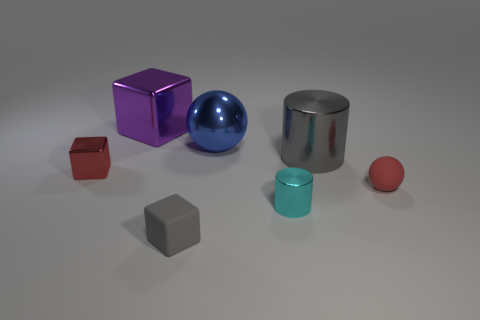
\includegraphics[width=.8\linewidth]{figures/CLEVR_example.png}
    \caption{Example of a generated image in the CLEVR dataset}
    \label{fig:clevr-example}
\end{figure}

Furthermore, the dataset contains information about each scene.
This includes all selected attributes for each object as well as the exact position of the centers of all the objects, both 3D-coordinates in the 3D scene and 2D-coordinates in the final rendered image.
In addition, simple spatial relations (in front of, behind, left, right) between the objects are calculated and stored.
These are simply based on the 3D-coordinates of the objects in relation to the position of the camera.


\subsection{Feature extractors}
To extract features from the images, I make use of different deep neural network architectures that are developed for this task.
First, I use the \cmtDK{why ResNet/VGG?} VGG19 \citep{Simonyan2015} which is an architecture based on many convolutional layers.
After the convolutional layers, the data is passed first through an average pooling layer which outputs 512x7x7 dimensions.
Next follow three linear layers with \emph{ReLU} non-linearities in between.
After flattening the input, these classification layers output 4069, 4069 and 1000 dimensions respectively.

Secondly, I include the ResNet-101 \citep{He2016} that tries to overcome problems of very deep networks, using \cmtDK{needs to be explained deeper?}{residual blocks}.
There are four blocks that output 256x56x56, 512x28x28, 1024x14x14 and 2048x1x1 dimensions.
A following average pooling layer outputs 2048x1x1 dimensions as well.
The final linear layer reduces the flattened data to 1000 dimensions, corresponding to the ImageNet classes.

Both architectures are available pretrained on an image classification task on the ImageNet dataset.
Since the task in this research is very different from a classification, multiple different adaptions of these architectures are compared. \cmtDK{deeper discussion about different layers of these networks}
Table \ref{tab:feature-extractor-archs} lists the different adaptions for both VGG19 and ResNet-101 that will be used in this research.
In the later chapters, it will be referred to these adaptions using the name in the table.

\begin{table}[h]
    \centering
    \begin{tabular}{rlc}
        \toprule
                            & \textbf{description}                                            & \textbf{ output dimensions } \\\midrule
        \textbf{VGG-0}      & contains only the convolutional layers                          & 512x7x7                      \\
        \textbf{VGG-avg}    & contains an additional average pooling layer                    & 512x7x7                      \\
        \textbf{VGG-cls1}   & \makecell[cl]{contains an additional one classification layer,                                 \\ including its non-linearity} & 4069                         \\
        \textbf{VGG-cls2}   & \makecell[cl]{contains another additional classification layer,                                \\ including its non-linearity} & 4069                         \\
        \textbf{VGG-cls3}   & the original VGG19 architecture                                 & 1000                         \\\midrule
        \textbf{ResNet-1}   & contains one residual block                                     & 256x56x56                    \\
        \textbf{ResNet-2}   & contains two residual blocks                                    & 512x28x28                    \\
        \textbf{ResNet-3}   & contains three residual blocks                                  & 1024x14x14                   \\
        \textbf{ResNet-4}   & contains four residual blocks                                   & 2048x1x1                     \\
        \textbf{ResNet-avg} & contains an additional average pooling layer                    & 2048x1x1                     \\
        \textbf{ResNet-cls} & the original ResNet-101 architecture                            & 1000                         \\
        \bottomrule
    \end{tabular}
    \caption{Different adaptions of VGG19 and ResNet-101 used in this research}
    \label{tab:feature-extractor-archs}
\end{table}

Furthermore, I experimented with both the pretrained models as well as with the architectures trained from scratch with a random initialization for the weights.
This reason for this was to test if the success of an experiment was actually making use of the pretrained knowledge incorporated in the models.
If that was not the case, the agents were likely not using image features, but instead relying on some other underlying patterns to solve the task.
Basically, this approach works as an indicator to determine the actual success of the agents aside from measures as the accuracy or precision.


\subsection{EGG}

\subsection{Ethical considerations}